\documentclass[11pt,a4paper]{article}
\usepackage[a4paper,top=10mm,bottom=10mm,left=14mm,right=14mm]{geometry}
\usepackage[T1]{fontenc}
\usepackage{amsmath}
\usepackage{amssymb}
\usepackage{enumitem}
\usepackage{multicol}
\usepackage{array}
\usepackage[table]{xcolor}
\usepackage{tikz}
\usepackage[most]{tcolorbox}
\usetikzlibrary{arrows.meta,decorations.pathreplacing}

% ================================================================
% Sequences and equations: an extension sheet.
%
% For pupils who can find the nth term of a linear sequence and solve
% linear equations. Every equation on the sheet comes from a question
% about sequences, and each part brings in one kind of equation.
%
% Part 1 sets two nth terms equal to find where two sequences meet,
% which puts the unknown on both sides: two candles burning down, and
% one phone running down while another charges. It ends with sequences
% that never meet.
%
% Part 2 compares terms in different positions, which gives brackets:
% three terms of a linear sequence written in x, rows of matchstick
% houses beside rows of squares and triangles with more shapes in
% them, a fence with one more post than panels, and cells that triple
% each hour.
%
% Part 3 has sequences with n in the denominator: a minibus cost shared
% between n people, a pizza cut into n slices, the fraction of a garden
% path that is grey, a sequence of fraction bars, and a minibus and a
% coach that cost the same for each person.
%
% Part 4 finds an unknown nth term an+b from two of its terms, which
% gives simultaneous equations: stacks of cups and of chairs, two
% sequences an+5 and bn+6, the fence again, and a Fibonacci-type
% sequence. It ends with open tasks.
%
% Each part starts with a worked example, followed by the same layout
% with gaps, and then by questions with the layout taken away.
% Equations are solved by doing the same thing to both sides, with the
% operation written under both sides, never with a flow chart.
% Simultaneous equations are solved by elimination.
%
% n is a position in a sequence, so a solution that is not a positive
% whole number shows that a number is not a term, or that two
% sequences never have equal terms in the same position. Several
% questions turn on this.
%
% The answers are in a comment beside each question. Every picture is
% drawn from its numbers, so the pictures agree with the answers.
% The sheet is written on and is six sides of A4.
% ================================================================

\pagestyle{empty}
\setlength{\parindent}{0pt}
\setlength{\parskip}{3pt}
\setlength{\multicolsep}{3pt}
\setlength{\columnsep}{14pt}
\setlist[enumerate,1]{label=\textbf{Q\arabic*.}, leftmargin=*, itemsep=6pt, topsep=4pt, parsep=2pt}
\setlist[enumerate,2]{label=(\alph*), leftmargin=*, itemsep=4pt, topsep=3pt, parsep=1pt}
\newcolumntype{C}[1]{>{\centering\arraybackslash}m{#1}}

% A gap for one number in a sentence, and a longer line for an answer.
\newcommand{\gap}{\underline{\hspace{0.95cm}}}
\newcommand{\ansline}[1][2.2cm]{\underline{\hspace{#1}}}
% Space to work in, ending with a line for the answer.
\newcommand{\workspace}[1]{\par\vspace{#1}\hfill Answer: \ansline[3.5cm]\par}
% The strut that sets the height of a table row to be written in.
\newcommand{\rowstrut}{\rule[-1.9mm]{0pt}{5.8mm}}

% The idea each part is built on, stated once and boxed, and the
% worked example. The boxes are tinted only faintly, and the title bar
% is pale with coloured text, so that the sheet is cheap to print.
\newtcolorbox{keyidea}{colback=orange!3,colframe=orange!35,boxrule=0.6pt,
  left=6pt,right=6pt,top=3pt,bottom=3pt}
\newtcolorbox{wex}[1]{colback=blue!2,colframe=blue!30,boxrule=0.6pt,
  colbacktitle=blue!8,coltitle=blue!50!black,
  left=6pt,right=6pt,top=3pt,bottom=4pt,
  title={\bfseries\small Worked example: #1},fonttitle=\small,
  toptitle=1pt,bottomtitle=1pt}

% The section headings, kept tight so the parts do not eat the page.
\newcommand{\parttitle}[2]{%
  \vspace{1pt}
  {\color{blue!45!black}\rule{\linewidth}{1pt}}\\[1pt]
  {\large\bfseries Part #1: #2}\\[-6pt]
  {\color{blue!45!black}\rule{\linewidth}{0.4pt}}
  \par\vspace{-5pt}}

% ----------------------------------------------------------------
% Working for an equation solved by doing the same thing to both
% sides. The lines are lined up on the equals sign. Between two lines,
% \bsop writes the operation under both sides, \bsopgap leaves both
% operations blank to fill in, and \bsnote writes a step that changes
% the whole line, such as expanding brackets. \sidegap is a blank for
% one side of a line.
\newenvironment{working}
  {\(\renewcommand{\arraystretch}{1.06}\begin{array}{@{}r@{\;}c@{\;}l@{}}}
  {\end{array}\)}
\newcommand{\opstyle}[1]{\text{\footnotesize\color{blue!55!black}$#1$}}
\newcommand{\bsop}[1]{\opstyle{#1} & & \opstyle{#1}\\}
\newcommand{\opgap}{\rule{0pt}{4.3mm}\rule{0.9cm}{0.4pt}}
\newcommand{\bsopgap}{\opgap & & \opgap\\}
\newcommand{\bsnote}[1]{\multicolumn{3}{c}{\text{\footnotesize\color{blue!55!black}#1}}\\}
\newcommand{\sidegap}[1][1.7cm]{\rule{0pt}{5.3mm}\rule{#1}{0.4pt}}

% A worked example or question laid out with a picture or table on the
% left, the working on the right and a sentence underneath:
% \eqlayout{<left width>}{<left>}{<working>}{<sentence>}
\newcommand{\eqlayout}[4]{%
  \begin{minipage}[c]{#1\linewidth}\raggedright #2\end{minipage}\hfill
  \begin{minipage}[c]{\dimexpr0.98\linewidth-#1\linewidth\relax}\centering #3\end{minipage}\par\smallskip
  #4}

% The layout of Part 1, with the table of terms and the sentence under
% it on the left, and the working on the right:
% \meetlayout{<table>}{<working>}{<sentence>}
\newcommand{\meetlayout}[3]{%
  \begin{minipage}[c]{0.62\linewidth}\raggedright #1\par\medskip #3\end{minipage}\hfill
  \begin{minipage}[c]{0.36\linewidth}\centering #2\end{minipage}}

% ----------------------------------------------------------------
% Part 1. The terms of two sequences in positions 1 to 8, one sequence
% to a row. \termtable[<header>]{<name>}{<8 terms>}{<name>}{<8 terms>},
% with the terms separated by &. \hl shades a cell, to show where the
% two sequences meet.
\newcommand{\hl}[1]{\cellcolor{orange!18}#1}
\newcommand{\termtable}[5][1 & 2 & 3 & 4 & 5 & 6 & 7 & 8]{%
  {\setlength{\tabcolsep}{2pt}%
  \begin{tabular}{|C{1.95cm}|*{8}{C{0.72cm}|}}\hline
  {\small Position $n$} & #1\\\hline
  #2\rowstrut & #3\\\hline
  #4\rowstrut & #5\\\hline
  \end{tabular}}}

% A candle h cm tall, with its base at (x,0), drawn 1 cm to 0.07 cm:
% \candle{<x>}{<h>}{<name>}
\newcommand{\candle}[3]{%
  \begin{scope}[shift={(#1,0)}]
  \pgfmathsetmacro{\ch}{0.062*#2}
  \draw[fill=yellow!8,line width=0.5pt] (-0.16,0) rectangle (0.16,\ch);
  \draw (0,\ch) -- (0,\ch+0.08);
  \fill[orange!55] (0,\ch+0.05) .. controls (0.1,\ch+0.14) and (0.06,\ch+0.26) .. (0,\ch+0.34)
    .. controls (-0.06,\ch+0.26) and (-0.1,\ch+0.14) .. (0,\ch+0.05);
  \node[font=\scriptsize,above,inner sep=1pt] at (0,\ch+0.34) {#2\,cm};
  \node[font=\scriptsize,below,inner sep=2pt] at (0,0) {#3};
  \end{scope}}
% Candles A and B after a number of hours, on a shelf:
% \candlepair{<x>}{<hours>}{<height of A>}{<height of B>}
\newcommand{\candlepair}[4]{%
  \begin{scope}[shift={(#1,0)}]
  \draw[line width=0.8pt] (-0.42,0) -- (1.32,0);
  \candle{0}{#3}{A}\candle{0.9}{#4}{B}
  \node[font=\scriptsize\bfseries] at (0.45,-0.62) {After #2};
  \end{scope}}

% A phone battery that is p% charged, with its bottom left corner at
% (x,y): \battery{<x>}{<y>}{<p>}
\newcommand{\battery}[3]{%
  \begin{scope}[shift={(#1,#2)}]
  \draw[line width=0.6pt,rounded corners=1.5pt] (0,0) rectangle (1.1,0.42);
  \fill (1.1,0.12) rectangle (1.17,0.30);
  \fill[gray!30] (0.05,0.05) rectangle ({0.05+0.01*#3},0.37);
  \node[font=\scriptsize] at (0.55,0.21) {#3\%};
  \end{scope}}

% ----------------------------------------------------------------
% Matchstick pictures. In each of these the argument is the pattern
% number n.
\tikzset{
  stick/.style={line width=1.1pt,cap=round,shorten >=1.3pt,shorten <=1.3pt,
    -{Circle[length=3.2pt,width=3.2pt]}},
  dim/.style={{Stealth[length=3pt]}-{Stealth[length=3pt]},line width=0.5pt},
  lab/.style={font=\scriptsize,inner sep=1pt}}
\newcommand{\pic}[1]{\begin{tikzpicture}[baseline=(current bounding box.south)]#1\end{tikzpicture}}
% One matchstick from one point to another.
\newcommand{\stick}[2]{\draw[stick] (#1) -- (#2);}

% The 3 matchsticks that square k adds to a row of squares.
\newcommand{\squaregroup}[1]{%
  \stick{0.5*#1-0.5,0}{0.5*#1,0}\stick{0.5*#1-0.5,0.5}{0.5*#1,0.5}
  \stick{0.5*#1,0}{0.5*#1,0.5}}
% A row of n squares of matchsticks that share their sides: 3n+1.
\newcommand{\chainsquares}[1]{\pic{%
  \stick{0,0}{0,0.5}
  \foreach \k in {1,...,#1} {\squaregroup{\k}}}}

% The 5 matchsticks that house k adds to a row of houses.
\newcommand{\housegroup}[1]{%
  \stick{0.5*#1-0.5,0}{0.5*#1,0}\stick{0.5*#1-0.5,0.5}{0.5*#1,0.5}
  \stick{0.5*#1,0}{0.5*#1,0.5}
  \stick{0.5*#1-0.5,0.5}{0.5*#1-0.25,0.79}\stick{0.5*#1-0.25,0.79}{0.5*#1,0.5}}
% A row of n houses of matchsticks that share their walls: 5n+1.
\newcommand{\chainhouses}[1]{\pic{%
  \stick{0,0}{0,0.5}
  \foreach \k in {1,...,#1} {\housegroup{\k}}}}

% A strip of n triangles of matchsticks, pointing up and down in turn:
% 2n+1. The first matchstick is the left side of the first triangle,
% and each triangle adds a matchstick along the bottom or the top and
% one sloping matchstick.
\newcommand{\chaintriangles}[1]{\pic{%
  \stick{0,0}{0.29,0.5}
  \foreach \k in {1,...,#1} {
    \ifodd\k\relax
      \stick{0.29*\k-0.29,0}{0.29*\k+0.29,0}\stick{0.29*\k,0.5}{0.29*\k+0.29,0}
    \else
      \stick{0.29*\k-0.29,0.5}{0.29*\k+0.29,0.5}\stick{0.29*\k+0.29,0.5}{0.29*\k,0}
    \fi}}}

% Patterns 1, 2 and 3 of a picture sequence, labelled underneath.
\newcommand{\threepatterns}[3]{%
  \begin{tabular}{@{}c@{\hspace{10pt}}c@{\hspace{10pt}}c@{}}
    #1 & #2 & #3\\[-1pt]
    {\scriptsize Pattern 1} & {\scriptsize Pattern 2} & {\scriptsize Pattern 3}
  \end{tabular}}

% A fence of n panels, with a post at each end and a post between each
% pair of panels, so n+1 posts.
\newcommand{\fence}[1]{%
  \foreach \k in {1,...,#1} {
    \pgfmathsetmacro{\xl}{(\k-1)*1.06+0.16}
    \draw[fill=yellow!6,line width=0.5pt] (\xl,0.12) rectangle (\xl+0.9,0.72);
    \foreach \s in {1,...,4} {\draw[gray!70] (\xl+0.18*\s,0.12) -- (\xl+0.18*\s,0.72);}}
  \pgfmathtruncatemacro{\posts}{#1}
  \foreach \k in {0,...,\posts} {\draw[fill=gray!40,line width=0.5pt] (\k*1.06,0) rectangle (\k*1.06+0.16,0.92);}}

% ----------------------------------------------------------------
% Part 3. The cost of the 360 pound minibus shared equally between n
% people, as a bar cut into n equal shares.
\newcommand{\sharebar}[1]{%
  \pgfmathtruncatemacro{\share}{360/#1}
  \foreach \k in {1,...,#1} {
    \draw[fill=green!4,line width=0.5pt] ({2.6*(\k-1)/#1},0) rectangle ({2.6*\k/#1},0.36);
    \node[font=\scriptsize] at ({2.6*(\k-0.5)/#1},0.18) {\pounds\share};}}
% The bars for n = 1, 2, 3 and 4 people, one above another.
\newcommand{\sharebars}{%
  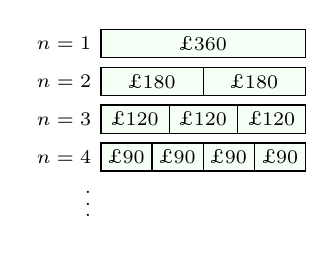
\begin{tikzpicture}[baseline=(current bounding box.center)]
  \foreach \p/\y in {1/0,2/-0.48,3/-0.96,4/-1.44} {
    \node[font=\scriptsize,left] at (0,\y+0.18) {$n=\p$};
    \begin{scope}[shift={(0,\y)}]\sharebar{\p}\end{scope}}
  \node[font=\scriptsize,left] at (0,-1.75) {$\vdots$};
  \end{tikzpicture}}

% A pizza cut into n equal slices, with the angle of one slice marked.
\newcommand{\pizza}[1]{\pic{%
  \pgfmathtruncatemacro{\ang}{360/#1}
  \draw[fill=yellow!10,line width=0.6pt] (0,0) circle (0.5);
  \ifnum#1>1
    \foreach \k in {1,...,#1} {\draw (0,0) -- ({90+360*\k/#1}:0.5);}
    \draw[line width=0.4pt] (90:0.13) arc (90:{90+360/#1}:0.13);
    \node[font=\tiny,inner sep=0pt] at ({90+180/#1}:0.3) {$\ang^\circ$};
  \else
    \node[font=\tiny,inner sep=0pt] at (0,0) {$\ang^\circ$};
  \fi}}

% Pattern n of the garden path: a row of n grey slabs with a border of
% white slabs, so 3 rows of n+2 slabs.
\newcommand{\gardenpath}[1]{\pic{%
  \pgfmathtruncatemacro{\w}{#1+2}
  \draw[black!70,line width=0.4pt,step=0.28] (0,0) grid ({0.28*\w},0.84);
  \foreach \c in {1,...,#1} {\filldraw[fill=gray!55,draw=black!70,line width=0.4pt]
    ({0.28*\c},0.28) rectangle ++(0.28,0.28);}}}

% Pattern n of the fraction bars: a bar cut into 2n+1 equal parts, with
% 2n-1 parts shaded. Every bar is the same length.
\newcommand{\fracbar}[1]{%
  \pgfmathtruncatemacro{\parts}{2*#1+1}
  \pgfmathtruncatemacro{\shaded}{2*#1-1}
  \foreach \k in {1,...,\parts} {
    \ifnum\k>\shaded\relax \def\barfill{white}\else \def\barfill{gray!40}\fi
    \draw[fill=\barfill,line width=0.5pt] ({2.8*(\k-1)/\parts},0) rectangle ({2.8*\k/\parts},0.3);}}

% The table for a picture sequence, with one \picrow for each row. The
% last column holds the nth term.
\newenvironment{pictable}{%
  \setlength{\tabcolsep}{2pt}%
  \begin{tabular}{|C{1.85cm}|*{6}{C{0.74cm}|}C{1.75cm}|}\hline
  {\small Pattern $n$} & 1 & 2 & 3 & 4 & 5 & 10 & {\small $n$th term}\\\hline}
  {\end{tabular}}
\newcommand{\picrow}[1]{{\small #1} & & & & & & & \rowstrut\\\hline}

% ----------------------------------------------------------------
% Part 4. A stack of n cups, drawn 1 cm to 0.1 cm. Each cup is 11 cm
% tall, and each cup added raises the top of the stack by 2 cm, so the
% stack is 2n+9 cm tall. The cups are drawn from the top of the stack
% down, so that each cup hides the part of the cup above it that sits
% inside it.
\newcommand{\cupstack}[1]{%
  \foreach \k in {#1,...,1} {
    \pgfmathsetmacro{\y}{0.2*(\k-1)}
    \draw[fill=white,line width=0.5pt] (-0.27,\y) -- (0.27,\y) -- (0.41,\y+1.1) -- (-0.41,\y+1.1) -- cycle;
    \draw[line width=1.1pt,line cap=round] (-0.44,\y+1.1) -- (0.44,\y+1.1);}}
% A stack of n chairs seen from the side, drawn 1 cm to 0.016 cm. Each
% chair is 85 cm tall, and each chair added raises the stack by 10 cm,
% so the stack is 10n+75 cm tall.
\newcommand{\chairstack}[1]{%
  \foreach \k in {1,...,#1} {
    \pgfmathsetmacro{\y}{0.16*(\k-1)}
    \draw[line width=0.7pt,line cap=round,line join=round]
      (0,\y) -- (0.08,\y+0.72) -- (0.86,\y+0.72) -- (0.94,\y)
      (0.08,\y+0.72) -- (0.02,\y+1.36);}}
% The height of a stack, marked beside it: \stackheight{<x>}{<top>}{<label>}
\newcommand{\stackheight}[3]{%
  \draw[dim] (#1,0) -- (#1,#2) node[midway,left,font=\scriptsize,inner sep=2pt] {#3};}

\begin{document}

\begin{center}
  {\Large\bfseries Sequences and Equations}\\[1pt]
  {\small Extension}
\end{center}
\vspace{-10pt}

% ================================================================
\parttitle{1}{When do two sequences meet?}

\begin{keyidea}
Two sequences have \textbf{equal terms in the same position} when their $n$th
terms are equal. We write one $n$th term equal to the other, and solve the equation
by doing the same thing to both sides. The solution $n$ is a position, so it must be
a positive whole number. If it is not, the sequences never have equal terms in the
same position.
\end{keyidea}

\begin{wex}{the sequences $5n+3$ and $3n+17$}
\meetlayout
  {\termtable[1 & 2 & 3 & 4 & 5 & 6 & \hl{7} & 8]
    {$5n+3$}{8 & 13 & 18 & 23 & 28 & 33 & \hl{38} & 43}
    {$3n+17$}{20 & 23 & 26 & 29 & 32 & 35 & \hl{38} & 41}}
  {\begin{working}
     5n+3 & = & 3n+17\\ \bsop{-3n}
     2n+3 & = & 17\\ \bsop{-3}
     2n & = & 14\\ \bsop{\div 2}
     n & = & 7
   \end{working}}
  {The terms in position \textbf{7} are equal.\par\smallskip
   Check: $5\times7+3=38$ and $3\times7+17=38$.}
\end{wex}

\begin{enumerate}
% 3n+2 = 26, 3n = 24, n = 8. Both 8th terms are 58.
\item Use the same method to find when the sequences $7n+2$ and $4n+26$ have equal terms.\par
\meetlayout
  {\termtable{$7n+2$}{9 & & & & & & &}{$4n+26$}{30 & & & & & & &}}
  {\begin{working}
     7n+2 & = & 4n+26\\ \bsop{-4n}
     \sidegap & = & \sidegap\\ \bsop{-2}
     \sidegap & = & \sidegap\\ \bsop{\div 3}
     n & = & \sidegap
   \end{working}}
  {The terms in position \gap\ are equal.\par\smallskip
   Check: \ansline[3.4cm] and \ansline[3.4cm].}

% 4n-4 = 20, 4n = 24, n = 6. Both 6th terms are 50.
\item Find when the sequences $9n-4$ and $5n+20$ have equal terms.\par
\meetlayout
  {\termtable{$9n-4$}{ & & & & & & &}{$5n+20$}{ & & & & & & &}}
  {\begin{working}
     9n-4 & = & 5n+20\\ \bsopgap
     \sidegap & = & \sidegap\\ \bsopgap
     \sidegap & = & \sidegap\\ \bsopgap
     n & = & \sidegap
   \end{working}}
  {The terms in position \gap\ are equal.\par\smallskip
   Check: \ansline[3.4cm] and \ansline[3.4cm].}

% (a) A: 30-2n, B: 21-n. (b) 30-2n = 21-n gives n = 9, when both are
% 12 cm. (c) A burns out first, after 15 hours. B lasts 21 hours.
\item \begin{minipage}[t]{0.5\linewidth}
  Two candles are lit at the same time. Candle A is 30\,cm tall and burns down
  by 2\,cm every hour. Candle B is 21\,cm tall and burns down by 1\,cm every hour.
  \begin{enumerate}
  \item Write an expression for the height of each candle after $n$ hours.\par
    A: \ansline[2.4cm] \quad B: \ansline[2.4cm]
  \end{enumerate}
  \end{minipage}\hfill
  \begin{minipage}[t]{0.47\linewidth}\raggedleft\vspace{0pt}
  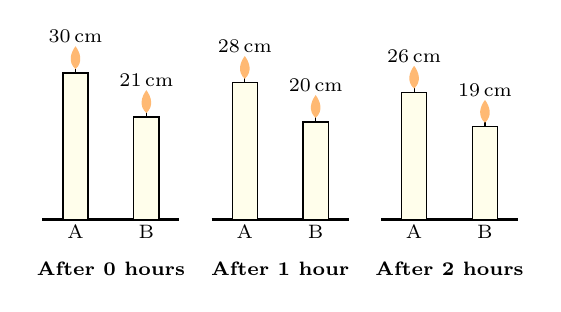
\begin{tikzpicture}[baseline=(current bounding box.north)]
    \candlepair{0}{0 hours}{30}{21}
    \candlepair{2.15}{1 hour}{28}{20}
    \candlepair{4.3}{2 hours}{26}{19}
  \end{tikzpicture}\end{minipage}
  \begin{enumerate}[start=2]
  \item Solve an equation to find when the two candles are the same height.
    How tall are they then?
    \workspace{1.6cm}
  \item Which candle burns out first? Explain how you know.\par\vspace{9pt}\hrulefill
  \end{enumerate}

% (a) Ella: 100-3n, Finn: 64+6n. (b) 100-3n = 64+6n gives 36 = 9n,
% n = 4, when both are at 88%.
\newpage
\item \begin{minipage}[t]{0.52\linewidth}
  Ella's phone is 100\% charged and loses 3\% of its charge every hour. Finn's
  phone is 64\% charged and is charging, so it gains 6\% every hour.
  \begin{enumerate}
  \item Write an expression for the charge of each phone after $n$ hours.\par
    Ella: \ansline[2.2cm] \quad Finn: \ansline[2.2cm]
  \item After how many hours do the two phones have the same charge?
  \end{enumerate}
  \end{minipage}\hfill
  \begin{minipage}[t]{0.45\linewidth}\raggedleft\vspace{0pt}
  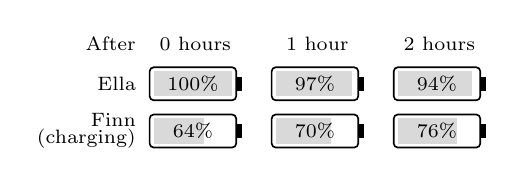
\begin{tikzpicture}[baseline=(current bounding box.north)]
    \foreach \h/\x in {0 hours/0,1 hour/1.55,2 hours/3.1} {
      \node[font=\scriptsize] at (\x+0.58,0.72) {\h};}
    \node[font=\scriptsize,left] at (-0.05,0.72) {After};
    \node[font=\scriptsize,left] at (-0.05,0.21) {Ella};
    \node[font=\scriptsize,left,align=right] at (-0.05,-0.39) {Finn\\[-2pt](charging)};
    \battery{0}{0}{100}\battery{1.55}{0}{97}\battery{3.1}{0}{94}
    \battery{0}{-0.6}{64}\battery{1.55}{-0.6}{70}\battery{3.1}{-0.6}{76}
  \end{tikzpicture}\end{minipage}
  \workspace{2.6cm}

% (a) 2n = 7, n = 3.5, which is not a whole number. (b) Both go up by 6
% each time, and 6n+5 is always 4 more than 6n+1. (c) 2n = c-1, so
% c = 3, 5, 7, ... Every possible c is an odd number of at least 3.
\item
  \begin{enumerate}
  \item Solve an equation to show that the sequences $4n+1$ and $2n+8$ never have
    equal terms in the same position.\par\vspace{2.5cm}
  \item Without solving an equation, explain why $6n+1$ and $6n+5$ never have
    equal terms in the same position. \hrulefill\par\vspace{9pt}\hrulefill
  \item The sequences $4n+1$ and $2n+c$ do have equal terms in the same position,
    where $c$ is a whole number. Find three possible values of $c$. What do all the
    possible values of $c$ have in common?\par\vspace{6pt}
    $c=$ \gap, \gap\ or \gap \qquad \hrulefill
  \end{enumerate}
\end{enumerate}

% ================================================================
\parttitle{2}{Comparing terms in different positions}

\begin{keyidea}
To write the term in position $n+4$ of the sequence $3n+1$, we replace $n$ with
$n+4$ to get $3(n+4)+1$. The brackets show that all of $n+4$ is multiplied by 3.
We expand the brackets first (remember $3(n+4)=3\times n+3\times4=3n+12$), and then
solve the equation by doing the same thing to both sides.
\end{keyidea}

\begin{wex}{houses and squares}
Sam makes a row of houses from matchsticks. Jo makes a row of squares, with 4 more
squares than Sam has houses. They use the same number of matchsticks. How many
houses does Sam make?\par\smallskip
\begin{minipage}[t]{0.49\linewidth}\centering
  \threepatterns{\chainhouses{1}}{\chainhouses{2}}{\chainhouses{3}}\par
  {\small Pattern $n$ has $n$ houses and $5n+1$ matchsticks.}
\end{minipage}\hfill
\begin{minipage}[t]{0.49\linewidth}\centering
  \threepatterns{\chainsquares{1}}{\chainsquares{2}}{\chainsquares{3}}\par
  {\small Pattern $n$ has $n$ squares and $3n+1$ matchsticks.}
\end{minipage}\par\medskip
\eqlayout{0.6}
  {Sam makes $n$ houses, which use $5n+1$ matchsticks.\par\smallskip
   Jo makes $n+4$ squares, which use $3(n+4)+1$ matchsticks.\par\smallskip
   The numbers of matchsticks are equal, so we write one equal to the other.}
  {\begin{working}
     5n+1 & = & 3(n+4)+1\\ \bsnote{expand the brackets}
     5n+1 & = & 3n+13\\ \bsop{-3n}
     2n+1 & = & 13\\ \bsop{-1}
     2n & = & 12\\ \bsop{\div 2}
     n & = & 6
   \end{working}}
  {Sam makes \textbf{6} houses and Jo makes \textbf{10} squares. Check: $5\times6+1=31$ and $3\times10+1=31$.}
\end{wex}

\begin{enumerate}[resume]
\newpage
% (a) The difference between each pair of terms is the same. (b)
% x+2 = 2x-4, x = 6. (c) 7, 15, 23; 8n-1.
\item The first three terms of a linear sequence are $x+1$, $2x+3$ and $4x-1$.
\begin{enumerate}
\item Explain why $(2x+3)-(x+1)=(4x-1)-(2x+3)$. \hrulefill
\item Solve the equation to find $x$. Then write the first three terms and the
  $n$th term of the sequence.
  \workspace{1.8cm}
\end{enumerate}

% Triangles: 2n+1. 5n+1 = 2(n+12)+1, 5n+1 = 2n+25, 3n+1 = 25, 3n = 24,
% n = 8. Ali makes 8 houses and Bea makes 20 triangles: 41 matchsticks.
\item Ali makes a row of houses. Bea makes a row of triangles, with 12 more triangles
than Ali has houses. They use the same number of matchsticks. How many houses does
Ali make?\par\smallskip
\begin{minipage}[t]{0.49\linewidth}\centering
  \threepatterns{\chainhouses{1}}{\chainhouses{2}}{\chainhouses{3}}\par
  {\small Pattern $n$ has $n$ houses and $5n+1$ matchsticks.}
\end{minipage}\hfill
\begin{minipage}[t]{0.49\linewidth}\centering
  \threepatterns{\chaintriangles{1}}{\chaintriangles{2}}{\chaintriangles{3}}\par
  {\small Pattern $n$ has $n$ triangles and \ansline[1.4cm] matchsticks.}
\end{minipage}\par\medskip
\eqlayout{0.6}
  {Ali makes $n$ houses, which use $5n+1$ matchsticks.\par\smallskip
   Bea makes \ansline[1.1cm] triangles, which use \ansline[1.9cm] matchsticks.\par\smallskip
   The numbers of matchsticks are equal, so we write one equal to the other.}
  {\begin{working}
     \sidegap & = & \sidegap[2.2cm]\\ \bsnote{expand the brackets}
     \sidegap & = & \sidegap\\ \bsop{-2n}
     \sidegap & = & \sidegap\\ \bsop{-1}
     \sidegap & = & \sidegap\\ \bsop{\div 3}
     n & = & \sidegap
   \end{working}}
  {Ali makes \gap\ houses and Bea makes \gap\ triangles. Check: \ansline[2.9cm] and \ansline[2.9cm].}

% (a) n panels and n+1 posts. (b) 25n+8(n+1) = 338, 33n+8 = 338,
% 33n = 330, n = 10. (c) 31n+4(n+1) = 25n+8(n+1), 35n+4 = 33n+8,
% n = 2. For 10 panels A costs 338 pounds and B costs 354 pounds, so A
% is cheaper.
\item \begin{minipage}[t]{0.6\linewidth}
  A fence has a post at each end and a post between each pair of panels. At
  garden centre A, a panel costs \pounds25 and a post costs \pounds8.
  \end{minipage}\hfill
  \begin{minipage}[t]{0.37\linewidth}\raggedleft\vspace{0pt}
  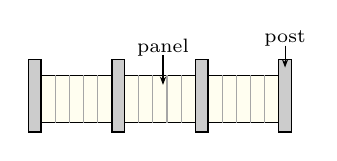
\begin{tikzpicture}[baseline=(current bounding box.north)]
    \fence{3}
    \node[lab,above] at (1.71,0.92) {panel};
    \draw[-{Stealth[length=3pt]},line width=0.4pt] (1.71,0.98) -- (1.71,0.6);
    \node[lab,above] at (3.26,1.05) {post};
    \draw[-{Stealth[length=3pt]},line width=0.4pt] (3.26,1.1) -- (3.26,0.82);
  \end{tikzpicture}\end{minipage}
  \begin{enumerate}
  \item Explain why a fence of $n$ panels costs $25n+8(n+1)$ pounds at garden centre A.
    \par\vspace{9pt}\hrulefill
  \item A fence from garden centre A costs \pounds338. How many panels does it have?
    \workspace{1.1cm}
  \item At garden centre B, a panel costs \pounds31 and a post costs \pounds4. For how
    many panels do the two garden centres charge the same? Which garden centre is
    cheaper for a fence of 10 panels?
    \workspace{1.4cm}
  \end{enumerate}

% (a) 9x-20 and 27x-65. (b) 27x-65 = 205, 27x = 270, x = 10.
\item A scientist grows cells in a dish. Every hour the number of cells triples, and
then 5 cells are taken out to be tested. There are $x$ cells at the start.\par
\begin{minipage}[t]{0.5\linewidth}
  \begin{enumerate}
  \item Complete the table. Expand the brackets in each term.
  \item After 3 hours there are 205 cells. How many cells were there at the start?
  \end{enumerate}
\end{minipage}\hfill
\begin{minipage}[t]{0.47\linewidth}\raggedleft\vspace{0pt}
  {\setlength{\tabcolsep}{3pt}\renewcommand{\arraystretch}{1.3}%
  \begin{tabular}{|l|C{0.55cm}|C{1.2cm}|C{2.3cm}|C{1.5cm}|}\hline
  {\small Hours} & 0 & 1 & 2 & 3\\\hline
  {\small Cells}\rowstrut & $x$ & $3x-5$ & $3(3x-5)-5$\newline${}=$\ansline[1.3cm] & \\\hline
  \end{tabular}}
\end{minipage}
\workspace{1.6cm}
\end{enumerate}

% ================================================================
\newpage
\parttitle{3}{The unknown in the denominator}

\begin{keyidea}
In some sequences the position $n$ is in the denominator of a fraction, such as
$\frac{360}{n}$. To solve an equation with $n$ in the denominator, we multiply both
sides by the denominator (remember $\frac{360}{n}\times n=360$). This gives an
equation with no fractions, which we solve by doing the same thing to both sides.
\end{keyidea}

\begin{wex}{sharing the cost of a minibus}
A minibus costs \pounds360 to hire for a day trip. The cost is shared equally
between the $n$ people who go, so each person pays $\frac{360}{n}$ pounds. How many
people must go for the cost to be \pounds24 each?\par\smallskip
\eqlayout{0.55}
  {\centering\sharebars}
  {\begin{working}
     \dfrac{360}{n} & = & 24\\[4pt] \bsop{\times n}
     360 & = & 24n\\ \bsop{\div 24}
     15 & = & n
   \end{working}}
  {\textbf{15} people must go. Check: $360\div15=24$.}
\end{wex}

\begin{enumerate}[resume]
% 360/n = 40, 360 = 40n, 9 = n. (b) 360/n = 25 gives n = 14.4, which is
% not a whole number, so no.
\item A pizza is cut into $n$ equal slices, so the angle of each slice is
$\frac{360}{n}$ degrees. How many slices must the pizza be cut into for each angle to
be $40^\circ$?\par\smallskip
\eqlayout{0.55}
  {\centering\threepatterns{\pizza{1}}{\pizza{2}}{\pizza{3}}\hspace{10pt}%
   \begin{tabular}[b]{@{}c@{}}\pizza{4}\\[-1pt]{\scriptsize Pattern 4}\end{tabular}}
  {\begin{working}
     \dfrac{360}{n} & = & 40\\[4pt] \bsop{\times n}
     \sidegap & = & \sidegap\\ \bsop{\div 40}
     \sidegap & = & n
   \end{working}}
  {\gap\ slices. Check: \ansline[3.4cm].}\par\medskip
Can a pizza be cut into equal slices with an angle of $25^\circ$? Solve an equation to
explain.\par\vspace{1.6cm}\hrulefill

% (a) Grey: 1,2,3,4,5,10; n. Total: 9,12,15,18,21,36; 3n+6.
% (b) n/(3n+6). (c) 10n = 3(3n+6), 10n = 9n+18, n = 18 (18/60 = 3/10).
% (d) 3n = 3n+6 gives 0 = 6, which is never true. There are 2n+6 white
% slabs, which is always more than twice the n grey slabs.
\item A garden path is made from a row of grey slabs with a border of white slabs.
\begin{enumerate}
\item Complete the table and write each $n$th term.\par
  \begin{minipage}[c]{0.4\linewidth}
  \threepatterns{\gardenpath{1}}{\gardenpath{2}}{\gardenpath{3}}
  \end{minipage}\hfill
  \begin{minipage}[c]{0.59\linewidth}\raggedleft
  \begin{pictable}\picrow{Grey slabs}\picrow{All slabs}\end{pictable}
  \end{minipage}
\item Write the fraction of the slabs in pattern $n$ that are grey. \ansline[2.5cm]
\item Which pattern has exactly $\frac{3}{10}$ of its slabs grey? Multiply both sides
  of your equation by 10 and by the denominator.
  \workspace{1.9cm}
\item Show that no pattern has exactly $\frac{1}{3}$ of its slabs grey. Use the picture
  to explain why.
  \vspace{1.5cm}\par\hrulefill
\end{enumerate}

% (a) (2n-1)/(2n+1). (b) 2n-1 = 0.92(2n+1), 0.16n = 1.92, n = 12, which
% is 23/25. (c) 2n-1 = 0.95(2n+1), 0.1n = 1.95, n = 19.5, so no.
% (d) It gets closer to 1, but there are always 2 parts not shaded.
\newpage
\item \begin{minipage}[t]{0.56\linewidth}
  Pattern $n$ of this sequence is a bar cut into $2n+1$ equal parts, with
  $2n-1$ of the parts shaded.
  \begin{enumerate}
  \item Write the fraction of the bar that is shaded in pattern $n$. \ansline[1.6cm]
  \end{enumerate}
  \end{minipage}\hfill
  \begin{minipage}[t]{0.42\linewidth}\raggedleft\vspace{0pt}
  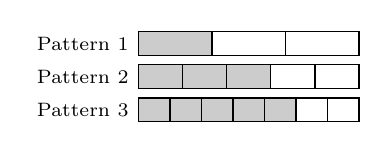
\begin{tikzpicture}[baseline=(current bounding box.north)]
  \foreach \p/\y in {1/0,2/-0.42,3/-0.84} {
    \node[font=\scriptsize,left] at (0,\y+0.15) {Pattern \p};
    \begin{scope}[shift={(0,\y)}]\fracbar{\p}\end{scope}}
  \end{tikzpicture}\end{minipage}
  \begin{enumerate}[start=2]
  \item Which pattern has $0.92$ of its bar shaded?
    \workspace{1.0cm}
  \item Is there a pattern with $0.95$ of its bar shaded? Explain.
    \vspace{0.8cm}\par\hrulefill
  \item What happens to the fraction shaded as $n$ gets larger? Use the picture to
    explain why it never reaches 1. \hrulefill
  \end{enumerate}

% 360/n = 600/(n+20), 360(n+20) = 600n, 360n+7200 = 600n, 7200 = 240n,
% n = 30. Each person pays 12 pounds on both.
\item A minibus costs \pounds360 to hire and a coach costs \pounds600. On a trip, the
coach carries 20 more people than the minibus, and each person pays the same amount.
How many people go on the minibus, and how much does each person pay?
\workspace{1.3cm}
\end{enumerate}

% ================================================================
\parttitle{4}{Finding an unknown \boldmath$n$th term}

\begin{keyidea}
The $n$th term of a linear sequence can be written as $an+b$, where $a$ and $b$ are
numbers. Two known terms give two equations in $a$ and $b$, called
\textbf{simultaneous equations} because the same $a$ and $b$ make both equations true.
When we subtract one equation from the other, the $b$s cancel out.
\end{keyidea}

\begin{wex}{a stack of cups}
A stack of 3 cups is 15\,cm tall, and a stack of 8 cups is 25\,cm tall. The height of a
stack of $n$ cups is $an+b$ centimetres. Find the $n$th term.\par\smallskip
\eqlayout{0.3}
  {\centering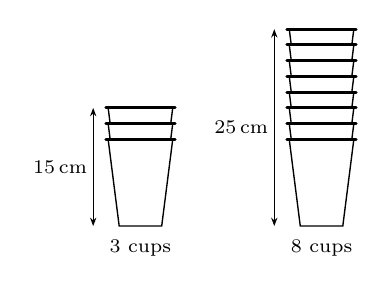
\begin{tikzpicture}[baseline=(current bounding box.center)]
    \cupstack{3}\stackheight{-0.6}{1.5}{15\,cm}
    \begin{scope}[shift={(2.3,0)}]\cupstack{8}\stackheight{-0.6}{2.5}{25\,cm}\end{scope}
    \node[font=\scriptsize,below] at (0,-0.05) {3 cups};
    \node[font=\scriptsize,below] at (2.3,-0.05) {8 cups};
  \end{tikzpicture}}
  {\begin{minipage}{\linewidth}
   \begin{minipage}[t]{0.5\linewidth}
   $\begin{array}[t]{@{}l@{\quad}r@{\;}c@{\;}l@{\quad}l@{}}
     \text{3 cups:} & 3a+b & = & 15 & (1)\\
     \text{8 cups:} & 8a+b & = & 25 & (2)
   \end{array}$\par\smallskip
   Subtract (1) from (2):\par\smallskip
   \hspace*{1.2cm}\begin{working}
     5a & = & 10\\ \bsop{\div 5}
     a & = & 2
   \end{working}
   \end{minipage}\hfill
   \begin{minipage}[t]{0.48\linewidth}
   Substitute $a=2$ into (1):\par\smallskip
   \hspace*{0.6cm}\begin{working}
     3\times2+b & = & 15\\
     6+b & = & 15\\ \bsop{-6}
     b & = & 9
   \end{working}
   \end{minipage}
   \end{minipage}}
  {The $n$th term is \textbf{\boldmath$2n+9$}. Each cup adds 2\,cm to the height.
   Check with (2): $8\times2+9=25$.}
\end{wex}

\begin{enumerate}[resume]
% 4a+b = 115, 10a+b = 175, 6a = 60, a = 10, 40+b = 115, b = 75. The nth
% term is 10n+75. (b) 10n+75 = 205, n = 13.
\item A stack of 4 chairs is 115\,cm tall, and a stack of 10 chairs is 175\,cm tall.
Find the $n$th term for the height of a stack of $n$ chairs.\par\smallskip
\eqlayout{0.3}
  {\centering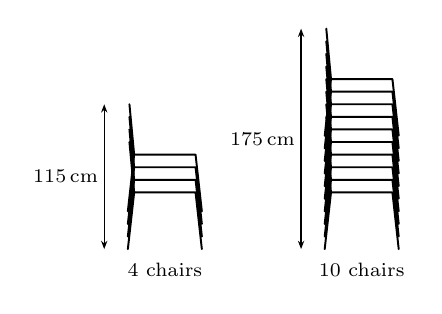
\begin{tikzpicture}[baseline=(current bounding box.center)]
    \chairstack{4}\stackheight{-0.3}{1.84}{115\,cm}
    \begin{scope}[shift={(2.5,0)}]\chairstack{10}\stackheight{-0.3}{2.80}{175\,cm}\end{scope}
    \node[font=\scriptsize,below] at (0.47,-0.05) {4 chairs};
    \node[font=\scriptsize,below] at (2.97,-0.05) {10 chairs};
  \end{tikzpicture}}
  {\begin{minipage}{\linewidth}
   \begin{minipage}[t]{0.5\linewidth}
   $\begin{array}[t]{@{}l@{\quad}r@{\;}c@{\;}l@{\quad}l@{}}
     \text{4 chairs:} & \sidegap[1.4cm] & = & \sidegap[1cm] & (1)\\
     \text{10 chairs:} & \sidegap[1.4cm] & = & \sidegap[1cm] & (2)
   \end{array}$\par\smallskip
   Subtract (1) from (2):\par\smallskip
   \hspace*{1.2cm}\begin{working}
     \sidegap[1.2cm] & = & \sidegap[1cm]\\ \bsop{\div 6}
     a & = & \sidegap[1cm]
   \end{working}
   \end{minipage}\hfill
   \begin{minipage}[t]{0.48\linewidth}
   Substitute $a=$ \gap\ into (1):\par\smallskip
   \hspace*{0.6cm}\begin{working}
     \sidegap[1.4cm] & = & \sidegap[1cm]\\
     \sidegap[1.4cm] & = & \sidegap[1cm]\\ \bsop{-40}
     b & = & \sidegap[1cm]
   \end{working}
   \end{minipage}
   \end{minipage}}
  {The $n$th term is \ansline[2cm]. Each chair adds \gap\,cm to the height.
   Check with (2): \ansline[3cm].}\par\medskip
How many chairs are in a stack that is 2.05\,m tall?
\workspace{0.6cm}

% (a) 3a+5 = 2b+6 gives 3a-2b = 1, and (a+5)+(b+6) = 18 gives a+b = 7.
% (b) 2a+2b = 14, add: 5a = 15, a = 3, b = 4. (c) 8, 11, 14, 17, 20
% and 10, 14, 18, 22, 26. (d) 4a+5 = 4b+6 gives 4(a-b) = 1, but
% 4(a-b) is a multiple of 4 when a and b are whole numbers.
\newpage
\item Two linear sequences have $n$th terms $an+5$ and $bn+6$. The 3rd term of $an+5$ is
equal to the 2nd term of $bn+6$, and the 1st terms of the two sequences add up to 18.
\begin{enumerate}
\item Show that $3a-2b=1$ and $a+b=7$. \hrulefill
\item Solve the simultaneous equations to find $a$ and $b$. Multiply $a+b=7$ by 2
  first, so that the $b$s cancel out when we add the equations.
  \workspace{2.8cm}
\item Write the first five terms of each sequence. \hfill \ansline[4cm] \quad \ansline[4cm]
\item Explain why, when $a$ and $b$ are whole numbers, the 4th terms of $an+5$ and
  $bn+6$ can never be equal. \hrulefill
\end{enumerate}

% 3p+4q = 138, 5p+6q = 222. 9p+12q = 414 and 10p+12q = 444, so p = 30
% and q = 12.
\item At garden centre C, a fence of 3 panels costs \pounds138 and a fence of 5 panels
costs \pounds222. Each fence has one more post than panels, as in Q8. Find the cost
of one panel and the cost of one post.
\workspace{3.0cm}

% x+y, x+2y, 2x+3y, 3x+5y. 2x+3y = 31 and 3x+5y = 50 give x = 5 and
% y = 7: 5, 7, 12, 19, 31, 50.
\item In a Fibonacci-type sequence, each term is the sum of the two terms before it.
Complete the table, then find $x$ and $y$ when the 5th term is 31 and the 6th term
is 50.\par\smallskip
{\setlength{\tabcolsep}{3pt}\renewcommand{\arraystretch}{1.3}%
\begin{tabular}{|l|*{6}{C{1.5cm}|}}\hline
{\small Term} & 1st & 2nd & 3rd & 4th & 5th & 6th\\\hline
{\small Value}\rowstrut & $x$ & $y$ & $x+y$ & & & \\\hline
\end{tabular}}
\workspace{2.6cm}

% Open. 3n+12 = 5n-2 gives n = 7. For example, Kai has 4 more boxes
% than Lily, with 3 pens in each, and Lily has n boxes of 5 pens but
% has given away 2 pens.
\item Write a real-life problem about two sequences that leads to the equation
$3(n+4)=5n-2$. Then solve your problem.
\par\vspace{2.2cm}\hrulefill\par\vspace{9pt}\hrulefill

% (a) Open. For example 4n+7 and 97-5n. (b) No. If an+b = cn+d when
% n = 10 and when n = 20, subtracting gives 10a = 10c, so a = c and
% then b = d, and the two sequences are the same.
\item
\begin{enumerate}
\item Design two sequences, one that goes up and one that goes down, that are equal
  at the 10th term with the value 47. Write their $n$th terms. \hfill
  \ansline[2.6cm] \quad \ansline[2.6cm]
\item Two different linear sequences have equal 10th terms. Can they also have equal
  20th terms? Explain.\par\vspace{1.9cm}\hrulefill
\end{enumerate}
\end{enumerate}

\end{document}
